\documentclass[titlepage = firstcover]{scrartcl}
\usepackage[aux]{rerunfilecheck}
\usepackage{fontspec}
\usepackage[main=ngerman, english, french]{babel}

% mehr Pakete hier
\usepackage{expl3}
\usepackage{xparse}

%Mathematik------------------------------------------------------
\usepackage{amsmath}   % unverzichtbare Mathe-Befehle
\usepackage{amssymb}   % viele Mathe-Symbole
\usepackage{mathtools} % Erweiterungen für amsmath
\usepackage{dsfont}
\usepackage[
  math-style=ISO,    % \
  bold-style=ISO,    % |
  sans-style=italic, % | ISO-Standard folgen
  nabla=upright,     % |
  partial=upright,   % /
]{unicode-math}% "Does exactly what it says on the tin."
\usepackage[section, below]{placeins}

% Laden von OTF-Mathefonts
% Ermöglich Unicode Eingabe von Zeichen: α statt \alpha

\setmathfont{Latin Modern Math}
%\setmathfont{Tex Gyre Pagella Math} % alternativ zu Latin Modern Math
\setmathfont{XITS Math}[range={scr, bfscr}]
\setmathfont{XITS Math}[range={cal, bfcal}, StylisticSet=1]

\AtBeginDocument{ % wird bei \begin{document}
  % werden sonst wieder von unicode-math überschrieben
  \RenewDocumentCommand \Re {} {\operatorname{Re}}
  \RenewDocumentCommand \Im {} {\operatorname{Im}}
}
\usepackage{mleftright}
\setlength{\delimitershortfall}{-1sp}
\usepackage[version=4]{mhchem}

%Sprache----------------------------------------------------------
\usepackage{microtype}
\usepackage{xfrac}
\usepackage[autostyle]{csquotes}    % babel
\usepackage[german, unicode, pdfusetitle]{hyperref}
\usepackage{bookmark}
\usepackage[shortcuts]{extdash}
%Einstellungen hier, z.B. Fonts
\usepackage{booktabs} % Tabellen

\setlength{\parindent}{0pt}

\title{V601 - Der Franck-Hertz Versuch}
\author{
  David Gutnikov\\
  \href{mailto:david.gutnikov@udo.edu}{david.gutnikov@udo.edu}\\
  Lasse Sternemann\\
  \href{mailto:lasse.sternemann@udo.edu}{lasse.sternemann@udo.edu}
}
\date{Bearbeitet am 7.07.2020}

\begin{document}
    \maketitle
    \newpage
    \tableofcontents
    \newpage

    \section{Auswertung}    
        \subsection{Mittlere freie Weglänge}
            Zunächst wird überprüft, ob die freie Weglänge $\overline{w}$ die Bedingung erfüllt, um ca. das tausendfache kleiner als der Abstand a zwischen Glühkathode und Beschleunigungsanode zu sein.
            Die freien Weglängen berechnen sich über Formel xx und werden daraufhin zur Berechnung des Verhältnis zwischen a=1cm und $\overline{w}$ genutzt.

            \begin{table}[h]
                \centering
                \caption{In der Tabelle sind die den Temperaturen zugehörigen mittleren Weglängen der Gasatome, sowie das zugehörige Verhältnis zur Beschleunigungsdistanz a zu sehen.}
                \label{tab:TabGasdruck}

                \begin{tabular}{c  c c}
                    \toprule
                    {$T \; [\text{K}] $} & {$\overline{w} \; [\text{m}\cdot 10^{-6}]$} &  {$\frac{\text{a}}{\overline{w}}$} \\
                    \midrule
                    300,85 & 4500 & 2,3 \\
                    424,15 & 5,8 &  1800  \\
                    443,15 & 2,9 &  3500  \\
                    470,25 & 1,2 &  8500  \\
                    \bottomrule
                \end{tabular}

            \end{table}

        \newpage
        \subsection{Differentielle Energieverteilung}
            Zunächst wird berechnet wie viel Volt ein Kästchen auf dem Graphen der jeweiligen Temperatur des xy-Schreibers entspricht. Dazu wird folgende Formel benutzt, die zunächst aus den 
            einzelnen Abständen $d_i$ den durchschnittlichen Abstand zwischen den 1 Volt Markierungen bestimmt und daraus die Volt pro Kästchen.

            \begin{equation*}
                \text{Volt/Kästchen} \; \text{[V]} = \sum_{i=1}^{n} \frac{1}{d_i}
            \end{equation*}

            \FloatBarrier

                \begin{figure}[h]
                  \centering
                  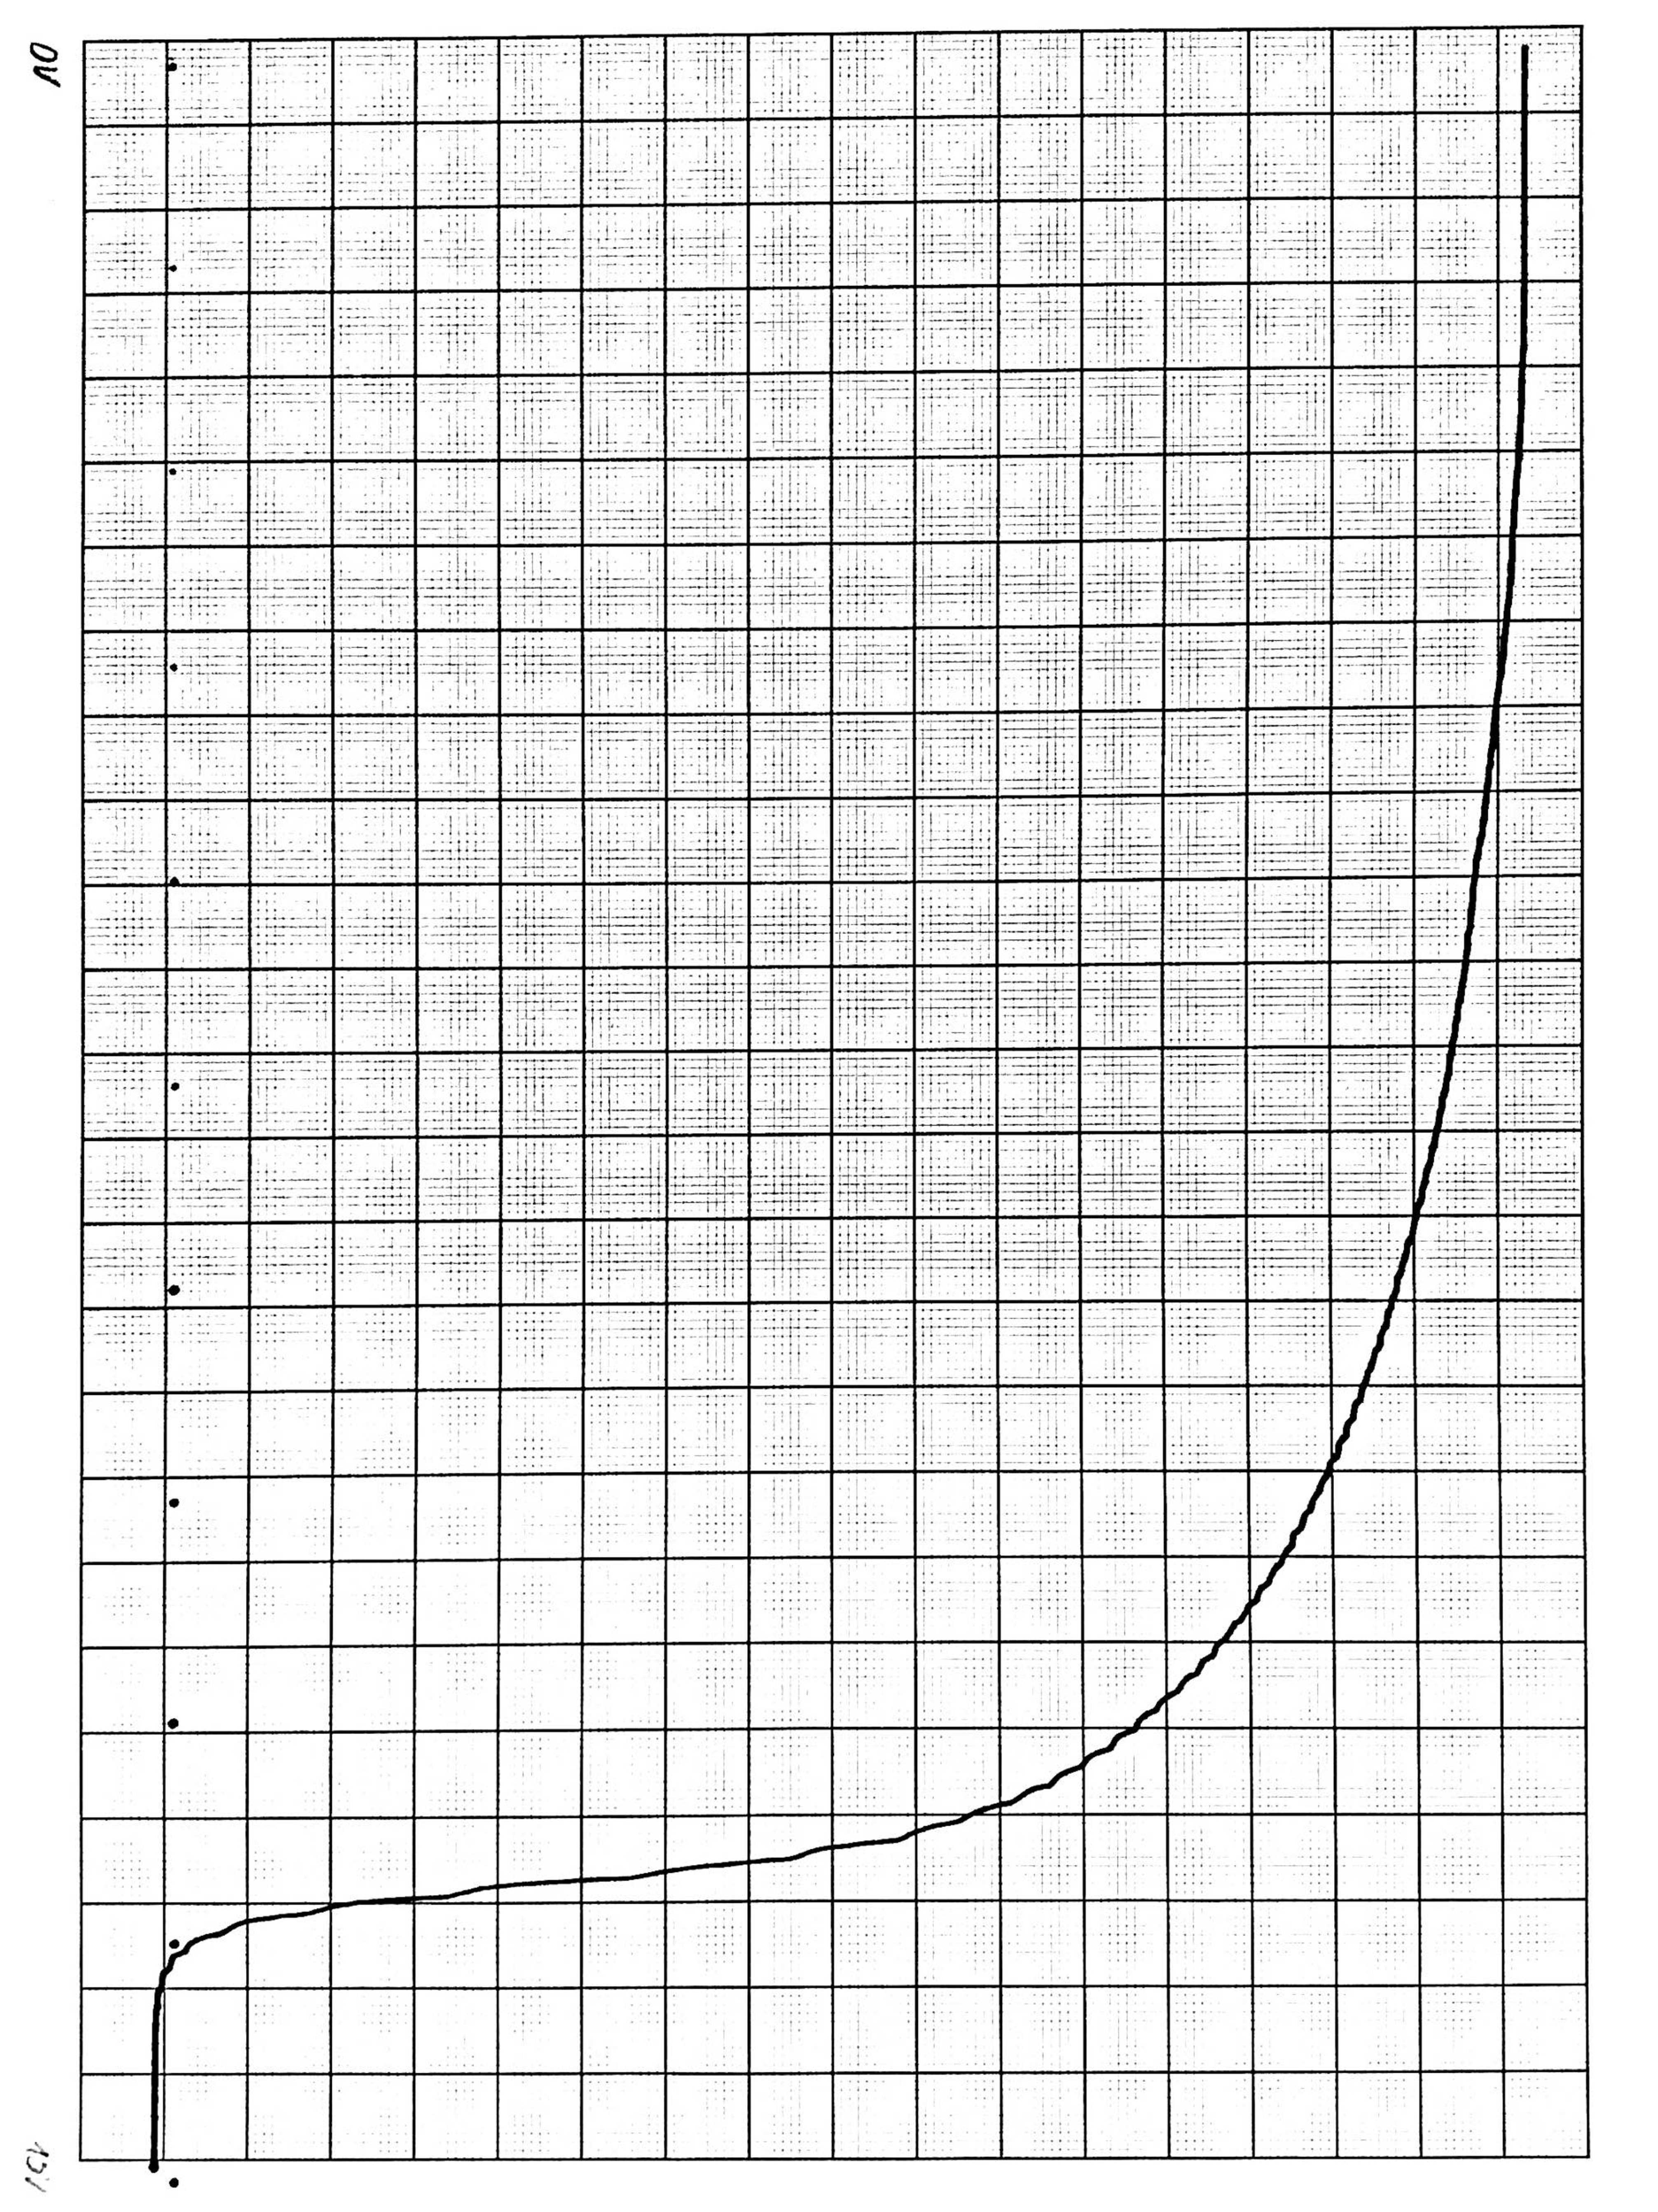
\includegraphics[width = 0.8\textwidth, angle=90]{T300.pdf}
                  \caption{In der Abbildung ist die integrale Energieverteilung der ausgelösten Elektronen bei einer Temperatur von 300,85 Kelvin zu sehen. Dazu wird der gemessene Kathodenstrom, der losgelösten Elektronen, in Abhängigkeit von der Bremsspannung aufgetragen. Der Abstand zwischen zwei schwarzen Punkten beträgt 1 Volt.}
                  \label{fig:Bild300}
                \end{figure}

                \begin{figure}[h]
                    \centering
                    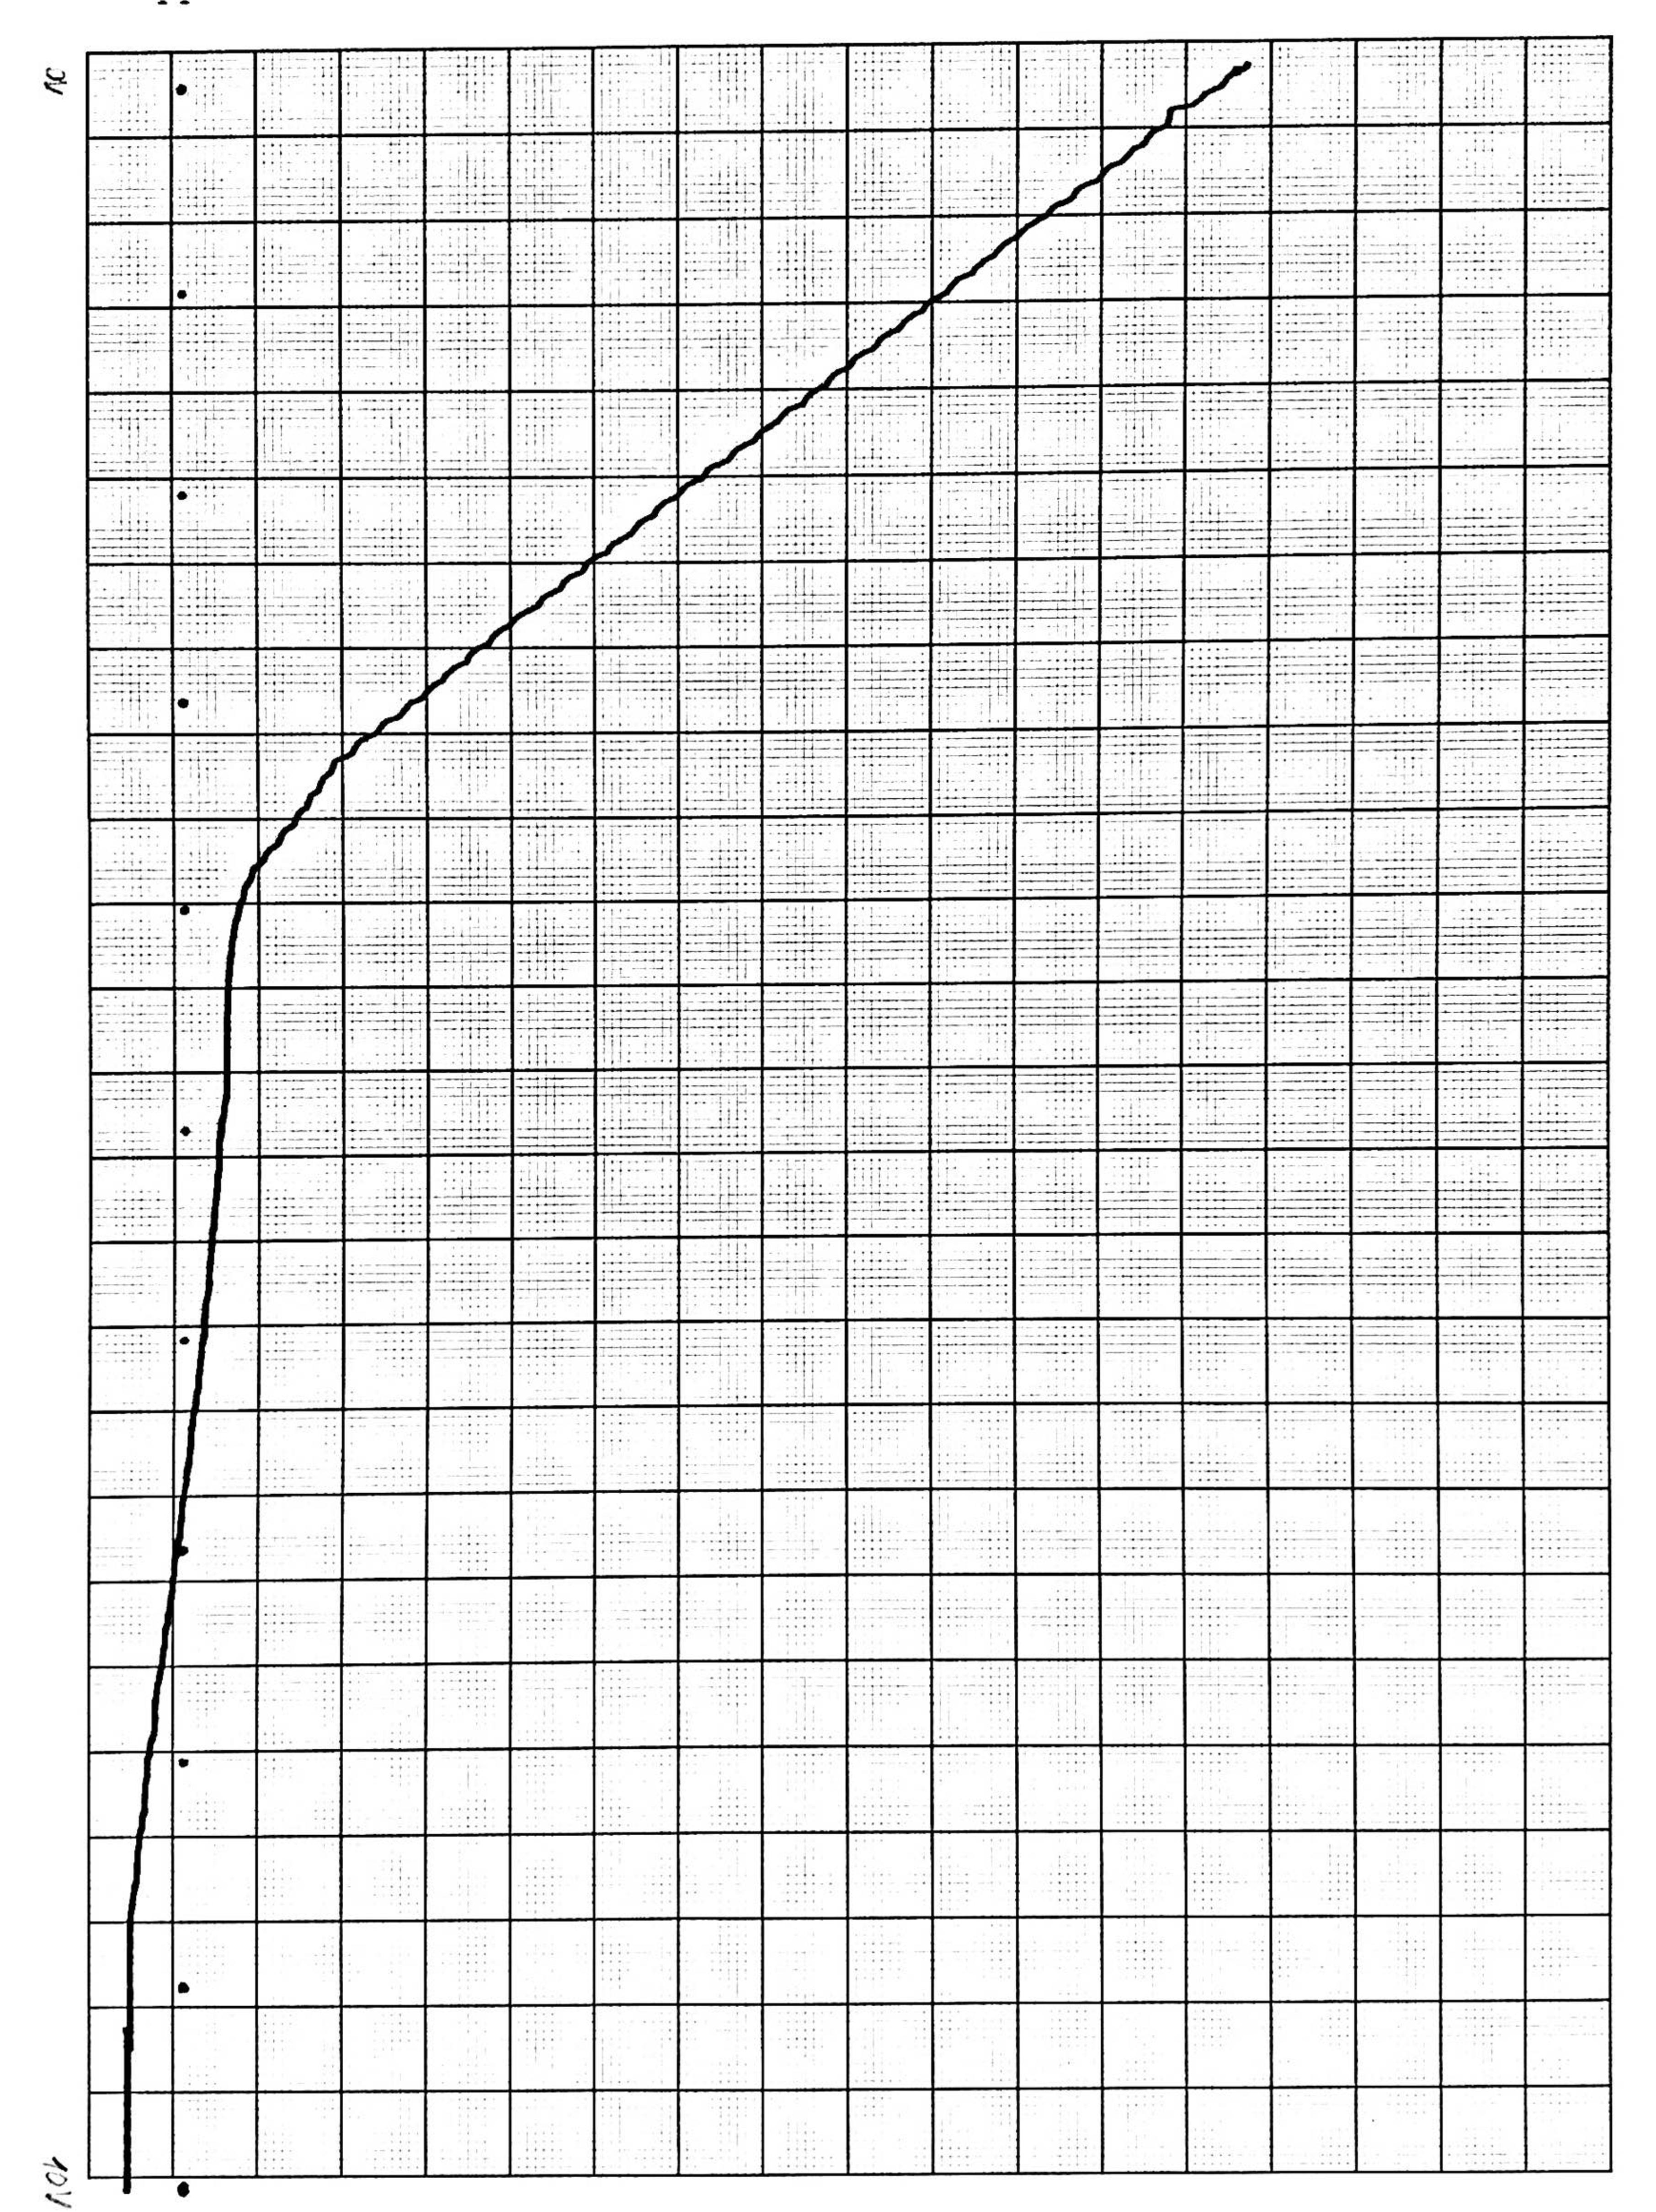
\includegraphics[width = 0.8\textwidth, angle=90]{T424.pdf}
                    \caption{In der Abbildung ist nun die integrale Energieverteilung der ausgelösten Elektronen bei einer Temperatur von 424,15 Kelvin zu sehen. Dazu wird der gemessene Kathodenstrom, der losgelösten Elektronen, erneut in Abhängigkeit von der Bremsspannung aufgetragen. Der Abstand zwischen zwei schwarzen Punkten beträgt wieder 1 Volt.}
                    \label{fig:Bild424}
                \end{figure}

            \FloatBarrier

            \noindent            

            \begin{table}[h]
                \centering
                \caption{In der Tabelle sind zunächst die Anzahlen der Kästchen zwischen den 1V-Markierungen zu sehen. Aus diesen wurde die durchschnittliche Skalierung der x-Achse in mV/Kästchen berechnet.}
                \label{tab:Tabelle1}

                \begin{tabular}{c c c c c}
                    \toprule
                    {} & {300,85 K} & {424,15 K} \\
                    \midrule
                    Kästchen/V    & 24 & 24 \\
                                  & 24 & 24 \\
                                  & 24 & 25 \\
                                  & 25 & 24 \\
                                  & 24 & 26 \\
                                  & 24 & 25 \\
                                  & 25 & 25 \\
                                  & 26 & 25 \\
                                  & 26 & 27 \\
                                  & 28 & 24 \\
                    \o \; mV/Kästchen & 40,1 & 40,2 \\
                    \bottomrule
                \end{tabular}

            \end{table}

            \FloatBarrier
            \noindent
            Nun kann für beide Temperaturen eine differentielle Energieverteilung aufgetragen werden, um das Kontaktpotential zwischen Glühkathode und Beschleunigungsanode zu bestimmen. Dazu werden 
            die Änderungen des Stroms pro Kästchen aus den Diagrammen des xy-Schreibers abgelesen und daraus die betragsmäßige Steigung berechnet. Diese betragsmäßige Steigung wird in Abhängigkeit
            der Bremsspannung für beide Temperaturen in den Grafiken \ref{fig:Steigung300} und \ref{fig:Steigung424} dargestellt. Die zugehörigen Werte befinden sich in der Tabelle 
            \ref{tab:Tabellexy} im Anhang.

            \FloatBarrier

                \begin{figure}[h]
                  \centering
                  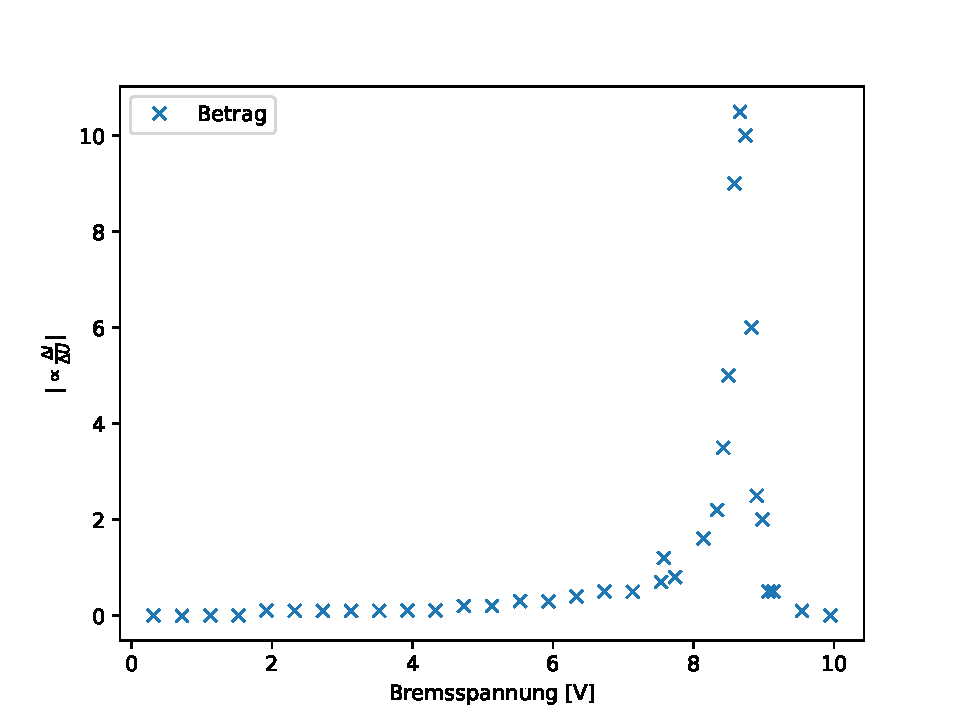
\includegraphics[width = 0.8\textwidth]{Steigung1.pdf}
                  \caption{In der Abbildung ist die differentielle Energieverteilung der ausgelösten Elektronen bei einer Temperatur von 300,85 Kelvin in Abhängigkeit von der Bremsspannung aufgetragen, an der Stelle der größten Steigung lässt sich das Kontaktpotential ablesen.}
                  \label{fig:Steigung300}
                \end{figure}

            \FloatBarrier

            \noindent

            Aus der obrigen Grafik \ref{fig:Steigung300} lässt sich ablesen, dass die Großzahl der Elektronen eine Energie von 8,7 eV besitzt. Da die Beschleunigungsspannung konstant 11 Volt beträgt,
            lässt sich das Kontaktpotential, welches nach der Theorie die Differenz dieser beiden Größen ist, als 2,3 Volt bestimmen.

            \FloatBarrier

                \begin{figure}[h]
                  \centering
                  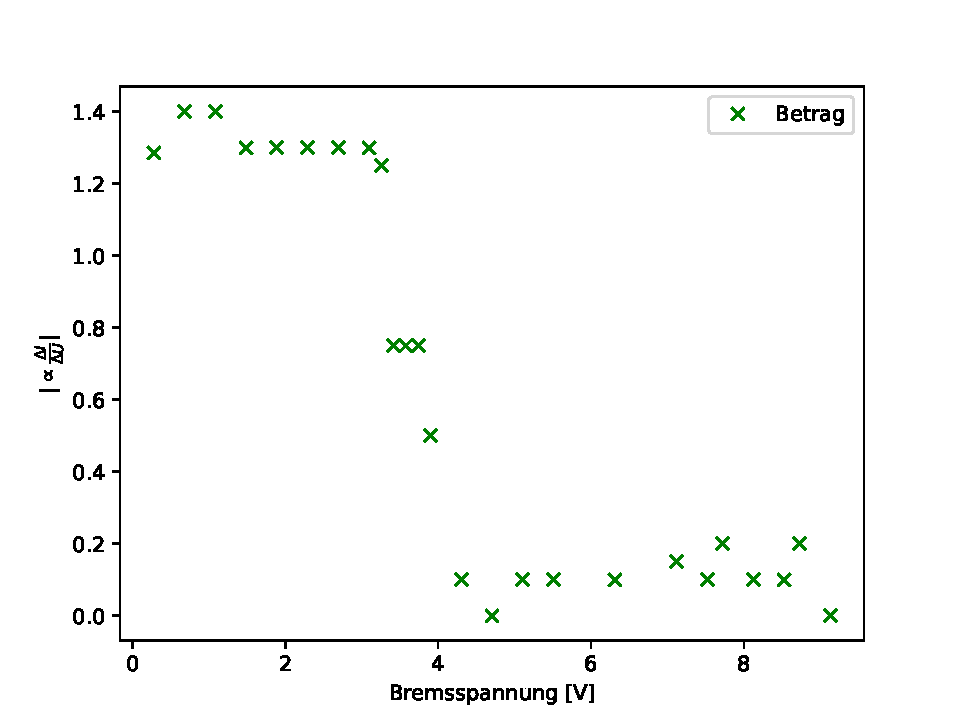
\includegraphics[width = 0.8\textwidth]{Steigung2.pdf}
                  \caption{In der Abbildung ist die differentielle Energieverteilung der ausgelösten Elektronen bei einer Temperatur von 424,15 Kelvin in Abhängigkeit von der Bremsspannung aufgetragen.}
                  \label{fig:Steigung424}
                \end{figure}

            \FloatBarrier

            \noindent

            In der Grafik zur Temperatur von 424,15 Kelvin \ref{fig:Steigung424} lässt sich ein solcher Peak nicht ausfindig machen, da die freie Weglänge nun stark eingeschränkt ist und elastische 
            Stöße die Geschwindigkeit bzw. Energie der Elektronen zufällig verändern. Das plötzliche Absinken geschieht, wenn die Energie der Elektronen genügt, um die Atome anzuregen. 
            Dabei verlieren sie ihre gesamte Energie, sodass nur wenige Atome mit einer höheren Energie gemessen werden können.

        \newpage
        \subsection{Die Franck-Hertz-Kurven}

            \FloatBarrier

                \begin{figure}[h]
                  \centering
                  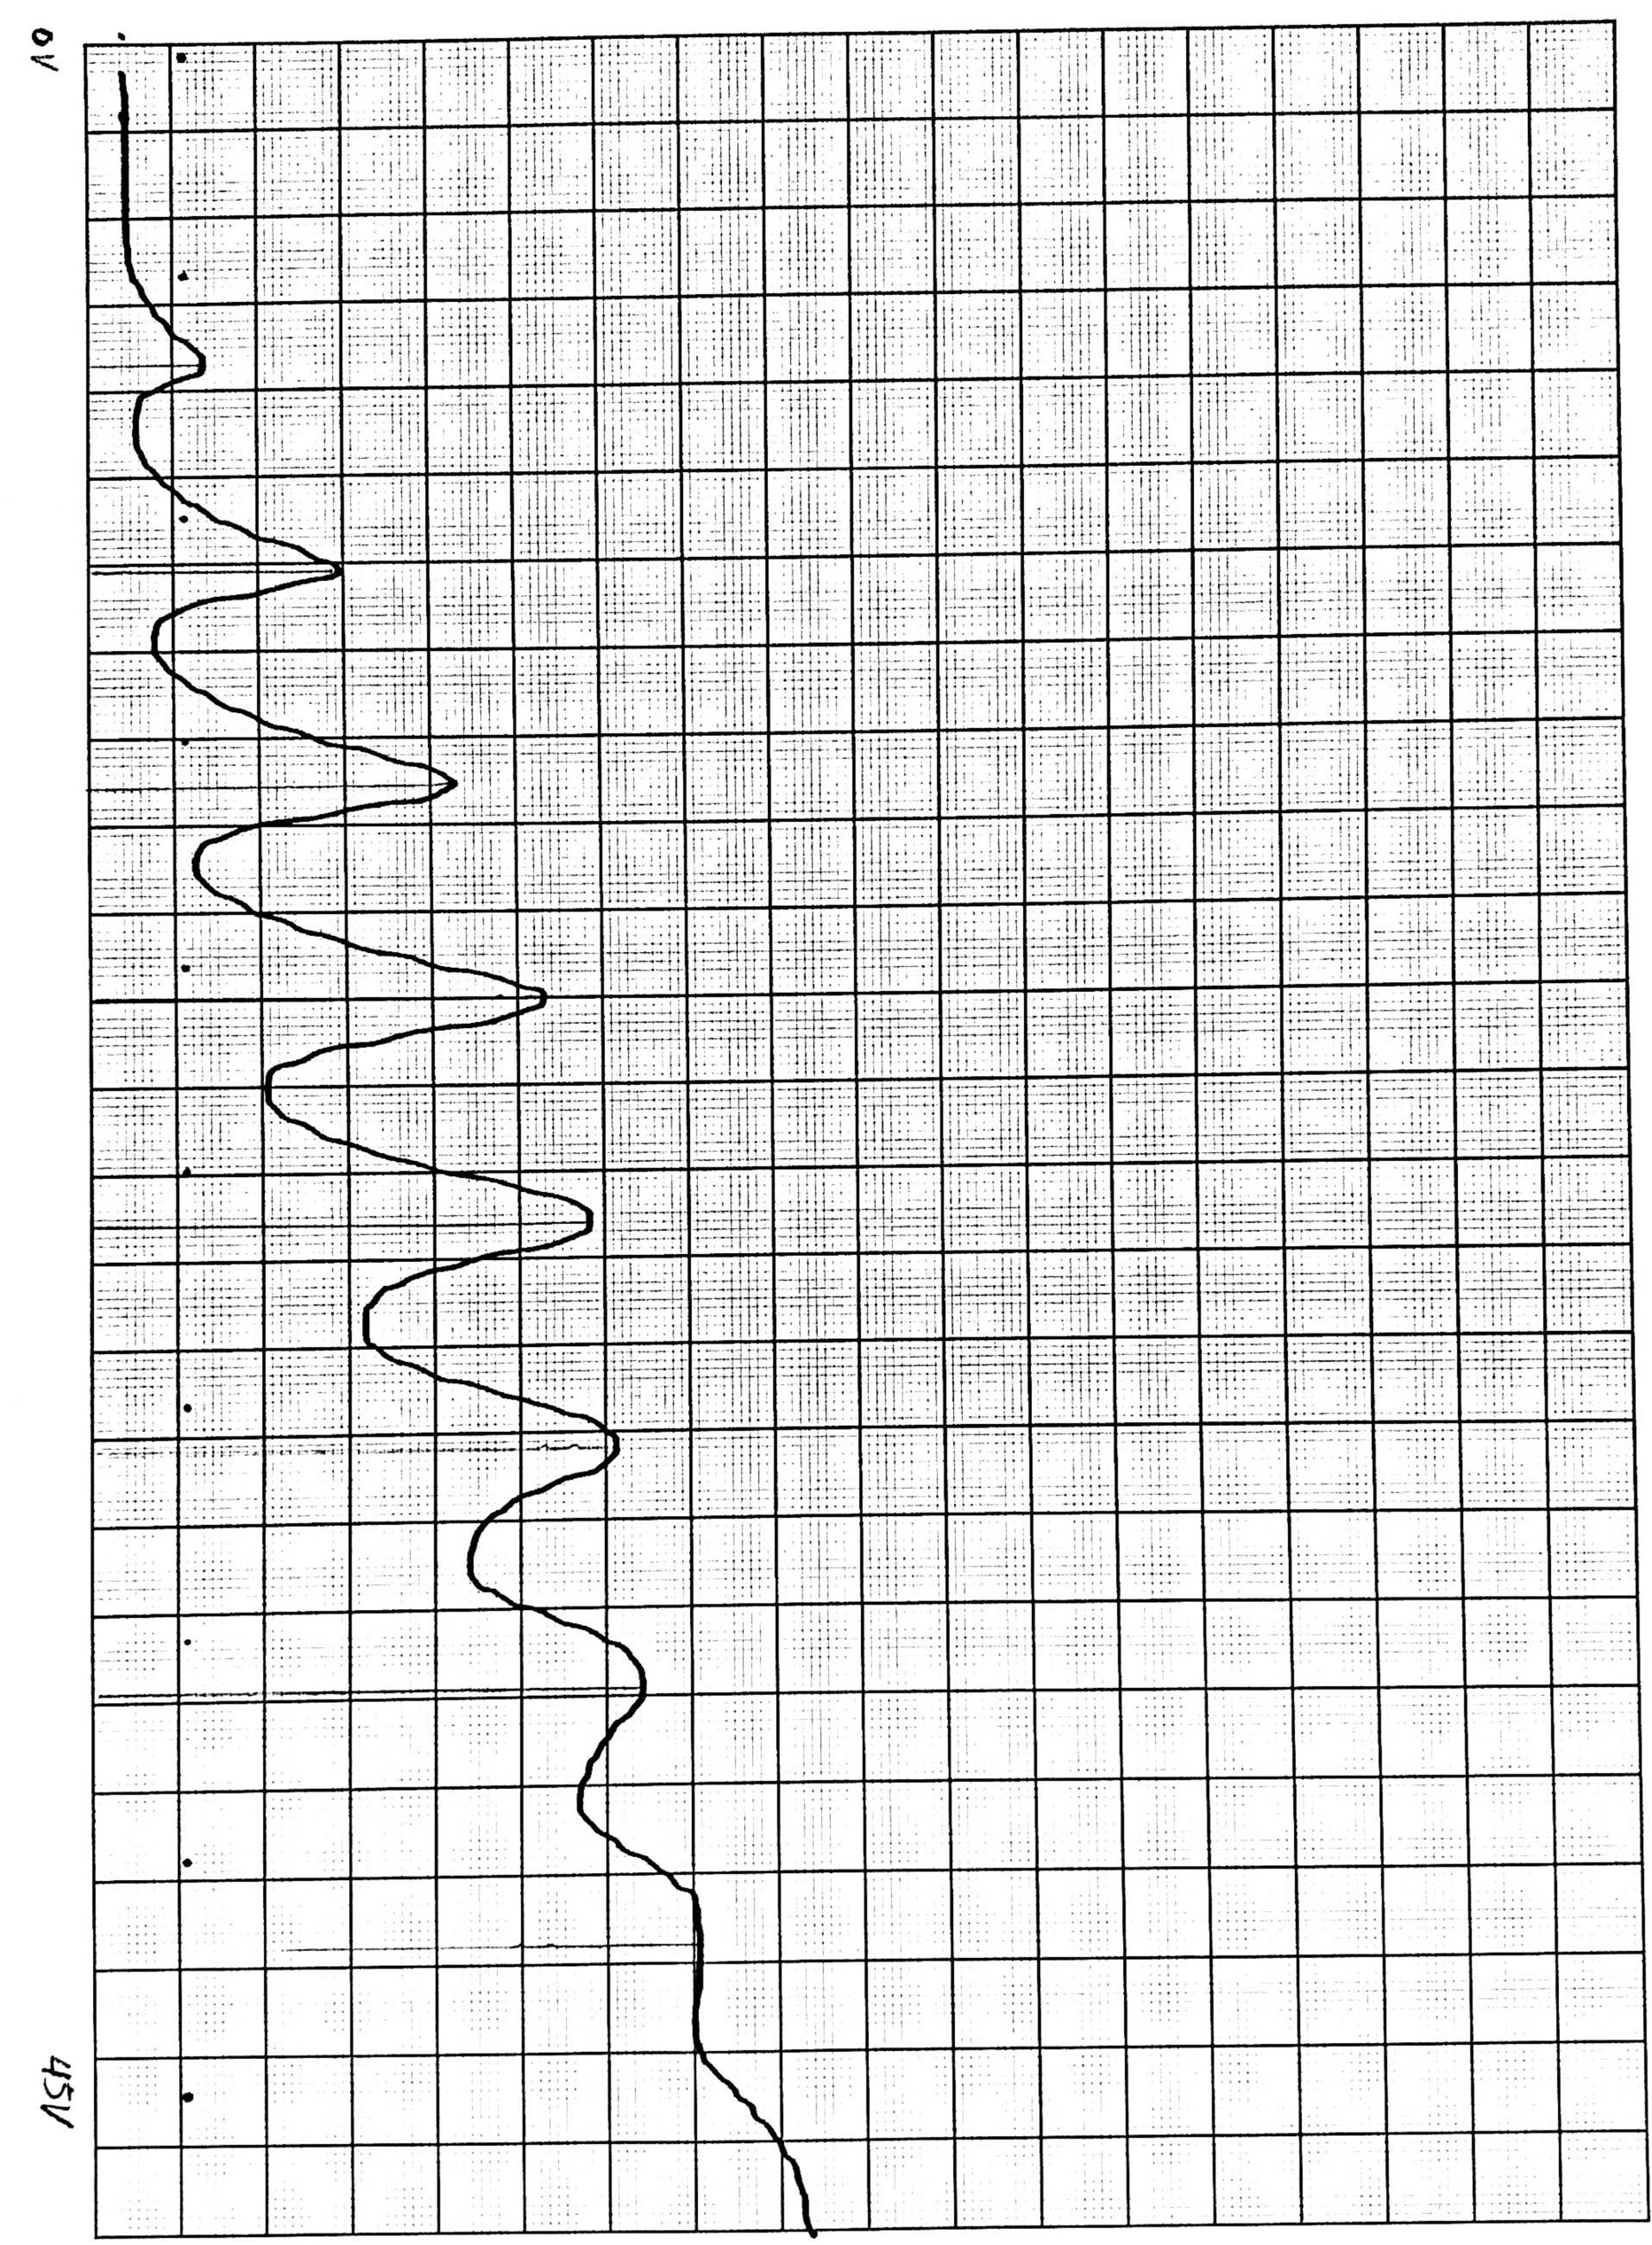
\includegraphics[width = 0.5\textwidth, angle=90]{HertzBild.pdf}
                  \caption{In der Abbildung ist die vom xy-Schreiber aufgenommene Franck-Hertz-Kurve bei einer Temeperatur von 470,25 Kelvin zu sehen.}
                  \label{fig:Steigung300}
                \end{figure}

            \FloatBarrier

            \noindent

            Zunächst wird mit dem selben Vorgehen wie im Abschnitt zur Energieverteilung der losgelösten Elektronen die x-Skala bestimmt. Der einzige Unterschied besteht darin, dass nun die Anzahl an
            Kästchen pro 5 Volt und nur die eine Temeperatur von 470,25 Kelvin betrachtet wird.


            \begin{table}[h]
                \centering
                \caption{In der Tabelle sind zunächst die Anzahlen der Kästchen zwischen den 5V-Markierungen zu sehen. Aus diesen wurde die durchschnittliche Skalierung der x-Achse in mV/Kästchen berechnet.}
                \label{tab:Tabelle1}

                \begin{tabular}{c c}
                    \toprule
                    {} & {470,25 K}  \\
                    \midrule
                    Kästchen/5V   & 24  \\
                                  & 27  \\
                                  & 25  \\
                                  & 25  \\
                                  & 23  \\
                                  & 26  \\
                                  & 26  \\
                                  & 24  \\
                                  & 26  \\
                    \o \; mV/Kästchen & 20,0  \\
                    \bottomrule
                \end{tabular}

            \end{table}

            \FloatBarrier
            \noindent
            Nun lässt sich der Abstand zwischen den Maxima der Kurve in Volt ablesen und somit die erste Ionisationsenergie der Quecksilberatome berechnen. Dazu wird Formel ref nach $\Delta E$ 
            umgestellt und es ergeben sich die folgenden Werte für die Ionisationsenergie. Zudem wird auch die Wellenlänge der Photonen berechnet, die ausgesendet werden, wenn die angeregten 
            Elektronen zurück in den Grundzustand springen.

            \begin{table}[h]
                \centering
                \caption{In der Tabelle ist der Abstand der Beschleunigungsspannung zwischen den Strommaxima, sowie die daraus berechnete Ionisationsenergie des Quecksilberatoms und die zugehörige Photonenwellenlänge beim Zurückspringen des angeregten Elektrons in die ursprüngliche Schale eingetragen.}
                \label{tab:TabelleHertz}

                \begin{tabular}{c c c}
                    \toprule
                    {$\Delta$ U [V]} & {$\Delta$ E [eV]} & {$\Delta \, \lambda$ [$\mu \text{m}$]} \\
                    \midrule
                        4,79 & 4,79 & 25,89 \\
                        4,99 & 4,99 & 24,85 \\
                        4,99 & 4,99 & 24,85 \\
                        5,19 & 5,19 & 23,89 \\
                        5,19 & 5,19 & 23,89 \\
                        5,39 & 5,39 & 23,01 \\
                        5,79 & 5,79 & 21,42 \\
                    \bottomrule
                \end{tabular}

            \end{table}

            \FloatBarrier
            \noindent
            Die durchschnittlichen Werte ergeben sich zu

            \begin{equation*}
                \overline{\Delta \text{U}} = 5,19 \, \text{V} \qquad \overline{\Delta \text{E}} = 5,19 \, \text{eV} \qquad \overline{\Delta \lambda} = 23.97 \, \mu \text{m.}
            \end{equation*}

        
    \newpage
    \section{Diskussion}
        Die Betrachtung der Messergebnisse zeigt eine deutliche Abweichung der Messergebnisse von 50 bis 100 Prozent zu den Literaturwerten. Dies lässt sich nicht direkt erklären. Ein möglicher 
        Störfaktor besteht darin, dass die Messung bei einer Temperatur von 470,25 Kelvin durchgeführt wurde. Dies führt zu einer eigentlich zu geringen mittleren Weglänge. Da die Minima und 
        Maxima dennoch gut zu erkennen sind, wurde die Messreihe bei dieser hohen Temperatur gewählt.






        \FloatBarrier
            
        \begin{table}[h]
          \centering
          \caption{In der Tabelle werden die Messwerte mit den Literaturwerten verglichen.}
        
          \begin{tabular}{c c c c}
              \toprule
              {Messgröße} & {Messwert} & {Literaturwert} & {Abweichung [\%]}\\
              \midrule
        
              $\Delta$U [V]                & 5,19    & 10,44  & 50,29 \%    \\
              $\Delta E_1$ [eV]             & 5,19  & 10,44 & 50,29 \%       \\
              $\Delta \lambda_1 $ [$\mu$m]   & 23,97     & 11,88  & 101.76 \%    \\
              Kontaktpotential [V]         & 2,3  & - &  -                  \\
              \bottomrule
          \end{tabular}
        \end{table}
  
        \FloatBarrier



    \section{Literaturverzeichnis}

            bkjsdfbkjdsfkjdfsjkjkfs


    \section{Anhang}

        \begin{table}[h]
            \centering
            \caption{In der Tabelle sind die aus dem Diagramm des xy-Schreibers abgelesenen Werte zur Bestimmung der differentiellen Energieverteilung eingetragen für die Temperaturen 300,85 Kelvin und 424,15 Kelvin.}
            \label{tab:Tabellexy}
           
            \begin{tabular}{c c c c c c}
                \toprule
                {$\Delta I_{300,85}$ [Kästchen]} & {$\Delta U_{300,85}$ [Kästchen]} & {$\frac{\Delta I}{\Delta U}$} & {$\Delta I_{424,15}$ [Kästchen]} & {$\Delta U_{424,15}$ [Kästchen]} & {$\frac{\Delta I}{\Delta U}$}\\
                \midrule
                    0 & 8 & 0 & 9 & 7 & 1,29\\
                    0 & 10 & 0 & 14 & 10 & 1,40\\
                    0 & 10 & 0 & 14 & 10 & 1,40\\
                    0 & 10 & 0 & 13 & 10 & 1,30\\
                    1 & 10 & 0,10 & 13 & 10 & 1,30\\
                    1 & 10 & 0,10 & 13 & 10 & 1,30\\
                    1 & 10 & 0,10 & 13 & 10 & 1,30\\
                    1 & 10 & 0,10 & 13 & 10 & 1,30\\
                    1 & 10 & 0,10 & 5 & 4 & 1,25\\
                    1 & 10 & 0,10 & 3 & 4 & 0,75\\
                    1 & 10 & 0,10 & 3 & 4 & 0,75\\
                    2 & 10 & 0,20 & 3 & 4 & 0,75\\
                    2 & 10 & 0,20 & 2 & 4 & 0,50\\
                    3 & 10 & 0,30 & 1 & 10 & 0,10\\
                    3 & 10 & 0,30 & 0 & 10 & 0\\
                    4 & 10 & 0,40 & 1 & 10 & 0,10\\
                    5 & 10 & 0,50 & 1 & 10 & 0,10\\
                    5 & 10 & 0,50 & 2 & 20 & 0,10\\
                    7 & 10 & 0,70 & 3 & 20 & 0,15\\
                    4 & 5 & 0,80 & 1 & 10 & 0,10\\
                    6 & 5 & 1,20 & 1 & 5 & 0,20\\
                    8 & 5 & 1,60 & 1 & 10 & 0,10\\
                    11 & 5 & 2,20 & 1 & 10 & 0,10\\
                    7 & 2 & 3,50 & 1 & 5 & 0,20\\
                    10 & 2 & 5,00 & 0 & 10 & 0\\
                    18 & 2 & 9,00 & & &\\
                    21 & 2 & 10,50 & & &\\
                    20 & 2 & 10,00 & & &\\
                    12 & 2 & 6,00 & & &\\
                    5 & 2 & 2,50 & & &\\
                    4 & 2 & 2,00 & & &\\
                    1 & 2 & 0,50 & & &\\
                    1 & 2 & 0,50 & & &\\
                    1 & 10 & 0,10 & & &\\
                    0 & 10 & 0 & & &\\

                \bottomrule
            \end{tabular}
           
        \end{table}
       
        \FloatBarrier
        \noindent


            
            
            
            


        \end{document}